% Options for packages loaded elsewhere
\PassOptionsToPackage{unicode}{hyperref}
\PassOptionsToPackage{hyphens}{url}
\PassOptionsToPackage{dvipsnames,svgnames,x11names}{xcolor}
%
\documentclass[
  10pt,
]{article}
\usepackage{amsmath,amssymb}
\usepackage{iftex}
\ifPDFTeX
  \usepackage[T1]{fontenc}
  \usepackage[utf8]{inputenc}
  \usepackage{textcomp} % provide euro and other symbols
\else % if luatex or xetex
  \usepackage{unicode-math} % this also loads fontspec
  \defaultfontfeatures{Scale=MatchLowercase}
  \defaultfontfeatures[\rmfamily]{Ligatures=TeX,Scale=1}
\fi
\usepackage{lmodern}
\ifPDFTeX\else
  % xetex/luatex font selection
\fi
% Use upquote if available, for straight quotes in verbatim environments
\IfFileExists{upquote.sty}{\usepackage{upquote}}{}
\IfFileExists{microtype.sty}{% use microtype if available
  \usepackage[]{microtype}
  \UseMicrotypeSet[protrusion]{basicmath} % disable protrusion for tt fonts
}{}
\makeatletter
\@ifundefined{KOMAClassName}{% if non-KOMA class
  \IfFileExists{parskip.sty}{%
    \usepackage{parskip}
  }{% else
    \setlength{\parindent}{0pt}
    \setlength{\parskip}{6pt plus 2pt minus 1pt}}
}{% if KOMA class
  \KOMAoptions{parskip=half}}
\makeatother
\usepackage{xcolor}
\usepackage[left=2cm, right=2cm, top=2cm, bottom=3cm, footskip = .5cm]{geometry}
\usepackage{longtable,booktabs,array}
\usepackage{calc} % for calculating minipage widths
% Correct order of tables after \paragraph or \subparagraph
\usepackage{etoolbox}
\makeatletter
\patchcmd\longtable{\par}{\if@noskipsec\mbox{}\fi\par}{}{}
\makeatother
% Allow footnotes in longtable head/foot
\IfFileExists{footnotehyper.sty}{\usepackage{footnotehyper}}{\usepackage{footnote}}
\makesavenoteenv{longtable}
\usepackage{graphicx}
\makeatletter
\def\maxwidth{\ifdim\Gin@nat@width>\linewidth\linewidth\else\Gin@nat@width\fi}
\def\maxheight{\ifdim\Gin@nat@height>\textheight\textheight\else\Gin@nat@height\fi}
\makeatother
% Scale images if necessary, so that they will not overflow the page
% margins by default, and it is still possible to overwrite the defaults
% using explicit options in \includegraphics[width, height, ...]{}
\setkeys{Gin}{width=\maxwidth,height=\maxheight,keepaspectratio}
% Set default figure placement to htbp
\makeatletter
\def\fps@figure{htbp}
\makeatother
\setlength{\emergencystretch}{3em} % prevent overfull lines
\providecommand{\tightlist}{%
  \setlength{\itemsep}{0pt}\setlength{\parskip}{0pt}}
\setcounter{secnumdepth}{5}
% Set up the fonts
\usepackage[urw-palatino]{mathdesign}
\usepackage[T1]{fontenc}


% Add accessibility support from http://www.richschwinn.com/accessibility
\RequirePackage{accsupp}
\RequirePackage{pdfcomment}
\newcommand{\AccTool}[2]{\BeginAccSupp{method=pdfstringdef,unicode,Alt={{#1}}}\pdftooltip{{#2}}{{#1}}\EndAccSupp{}}

% Set the language for 508
\hypersetup{
  pdftitle = {title},
  pdflang = en-US}

% Set up the headers and footers
\usepackage{graphicx}
\usepackage{fancyhdr}
\usepackage{ifthen}
\usepackage{everypage}
\usepackage{float}
\usepackage{subfig}

% Avoid struggling over figure and table float in Rmarkdown
\let\origfigure\figure
\let\endorigfigure\endfigure
\renewenvironment{figure}[1][2] {
    \expandafter\origfigure\expandafter[H]
} {
    \endorigfigure
}

\let\origtable\table
\let\endorigtable\endtable
\renewenvironment{table}[1][2] {
    \expandafter\origtable\expandafter[H]
} {
    \endorigtable
}

% First page has the large title and NOAA logo
\pagestyle{fancy}
\fancyhf{}
\setlength\headheight{40pt}
\fancyheadoffset[L]{0.5cm}
\cfoot{\thepage}

\fancyheadinit{%
   \ifthenelse{\value{page}=1}%
      {\fancyhead[R]{\textsf{\emph{24 March 2025}}}
       \fancyhead[L]{\textsf{\LARGE Mid-Atlantic EAFM Risk Assessment: 2025 Update}}
      }%
      {\fancyhead[R]{}
       \fancyhead[L]{\textsf{\emph{Risk Assessment Update 2025}}}
      }
}

\renewcommand{\headrulewidth}{0.4pt}
\renewcommand{\footrulewidth}{0pt}

% Make caption fonts a bit smaller
\usepackage[font={small}]{caption}


% Change section labels to san serif
\usepackage{sectsty}
\allsectionsfont{\normalfont\sffamily\bfseries}
\usepackage{booktabs}
\usepackage{longtable}
\usepackage{array}
\usepackage{multirow}
\usepackage{wrapfig}
\usepackage{float}
\usepackage{colortbl}
\usepackage{pdflscape}
\usepackage{tabu}
\usepackage{threeparttable}
\usepackage{threeparttablex}
\usepackage[normalem]{ulem}
\usepackage{makecell}
\usepackage{xcolor}
\ifLuaTeX
  \usepackage{selnolig}  % disable illegal ligatures
\fi
\usepackage{bookmark}
\IfFileExists{xurl.sty}{\usepackage{xurl}}{} % add URL line breaks if available
\urlstyle{same}
\hypersetup{
  colorlinks=true,
  linkcolor={Maroon},
  filecolor={Maroon},
  citecolor={Blue},
  urlcolor={blue},
  pdfcreator={LaTeX via pandoc}}

\author{}
\date{\vspace{-2.5em}}

\begin{document}

{
\hypersetup{linkcolor=}
\setcounter{tocdepth}{2}
\tableofcontents
}
\section{New England Risk Policy}\label{new-england-risk-policy}

The Risk Policy Statement and Concept (2025) outlines how the Council intends to operationalize environmental and socioeconomic considerations in management. The Council also highlights how they anticipate organizations, including the Northeast Fisheries Science Center (NEFSC), contributing to this effort. The NEFSC is expected to contribute through continued updates of the State of the Ecosystem report, and further development of risk indicators. Risk Policy Factors developed by the Council consider 1. Stock Status and Uncertainty, 2. Climate and Ecosystem Considerations, and 3. Economic and Community Importance. Factors related to Stock Status and Uncertainty are derived from stock assessments. Here we demonstrate how indicators from the State of the Ecosystem report and indicators developed for research track assessments could inform Climate and Ecosystem Considerations and Economic and Community Importance.

\subsection{Potential indicators for Climate and Ecosystem Considerations}\label{potential-indicators-for-climate-and-ecosystem-considerations}

In developing indicators for Climate and Ecosystem Considerations, we prioritized indicators with a statistically significant, mechanistic correlation with the life history they were designed to assess. We prioritized indicators which have not been included in the stock assessment to date to avoid redundant consideration of the indicator in management advice. We prioritized indicators from Term of Reference 1 (ToR1) from research track stock assessments as they have been collaboratively developed with stock assessment working groups and peer reviewed.

\textbf{American plaice indicators}

A research track assessment of American plaice was completed in 2022. TOR1 of the assessment identified multiple environmental indicators that are correlated with life history of American plaice. The most appropriate indicator for application in the Risk Policy is Annual mean bottom temperature anomaly. This indicator was significantly correlated with fall and spring mean latitude of American plaice in the NEFSC trawl survey, suggesting the species is distributed further North and East in warmer years compared to cooler years. Bottom temperature anomaly is regularly included in the State of the Ecosystem report. Details on this indicator are available in the SOE technical document.

\begin{center}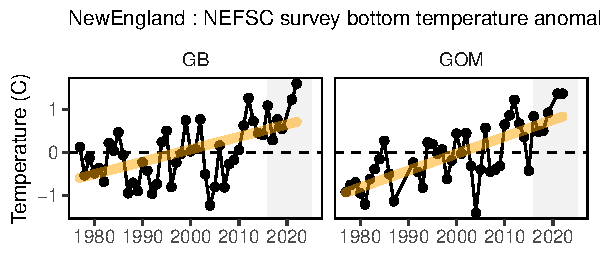
\includegraphics{NE_RiskPolicy_2025_DRAFT_files/figure-latex/plaice_eco-1} \end{center}

\textbf{Atlantic cod indicators}

\textbf{Atlantic herring indicators}

** Georges Bank Yellowtail flounder indicators**

\begin{center}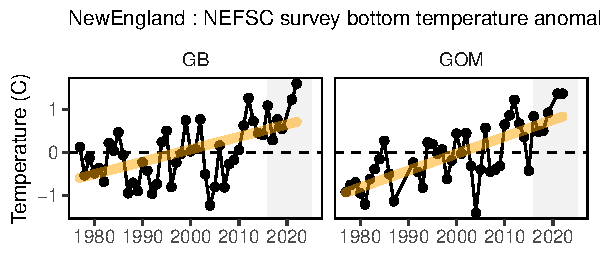
\includegraphics{NE_RiskPolicy_2025_DRAFT_files/figure-latex/gb_yt_eco-1} \end{center}

** Southern New England Yellowtail flounder indicators**

\begin{center}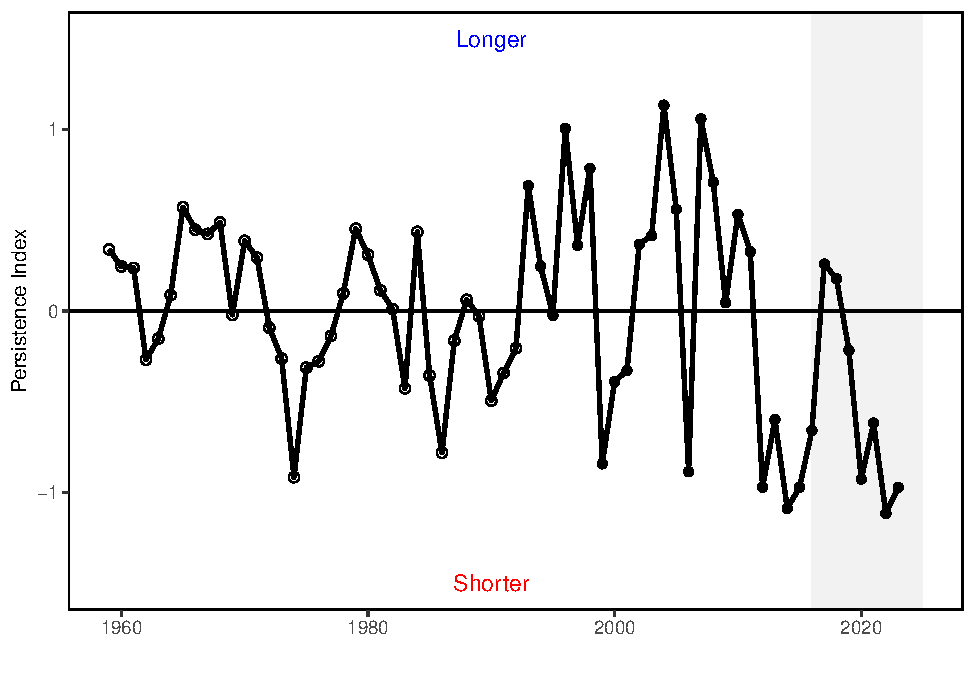
\includegraphics{NE_RiskPolicy_2025_DRAFT_files/figure-latex/sne_yt_eco-1} \end{center}

\subsection{Potential Indicators for Commercial Fishery Characterization}\label{potential-indicators-for-commercial-fishery-characterization}

\textbf{Commercial fishery characterization indicators}

\begin{figure}

{\centering 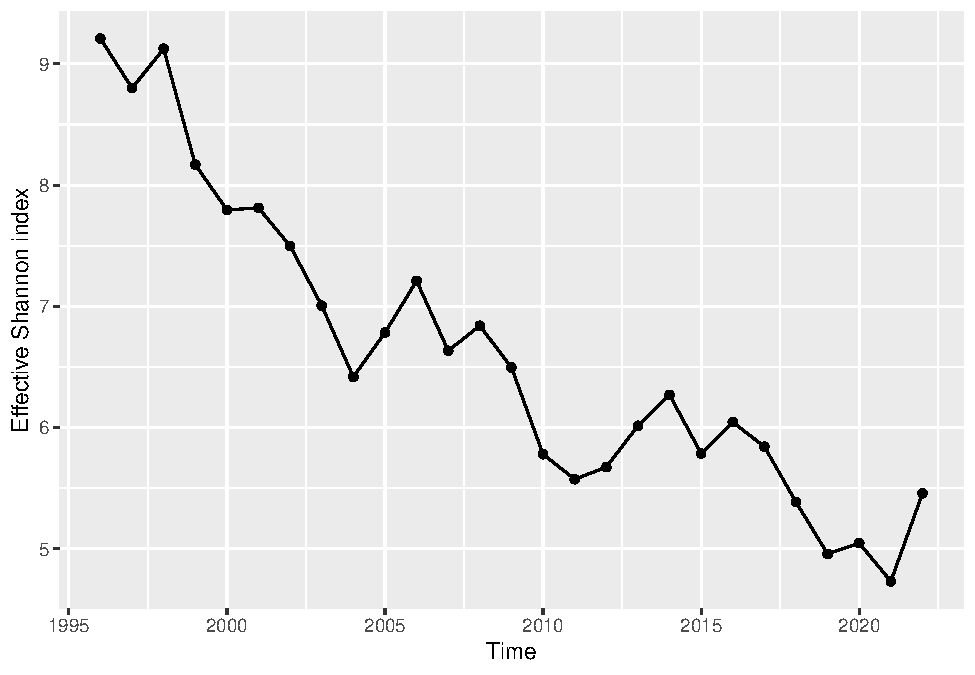
\includegraphics{NE_RiskPolicy_2025_DRAFT_files/figure-latex/comm-1} 

}

\caption{Effective Shannon index of NE commercial fisheries}\label{fig:comm}
\end{figure}

\subsection{Potential Indicators for Recreational Fishery Characterization}\label{potential-indicators-for-recreational-fishery-characterization}

\textbf{Recreational fishery characterization indicators}

\begin{center}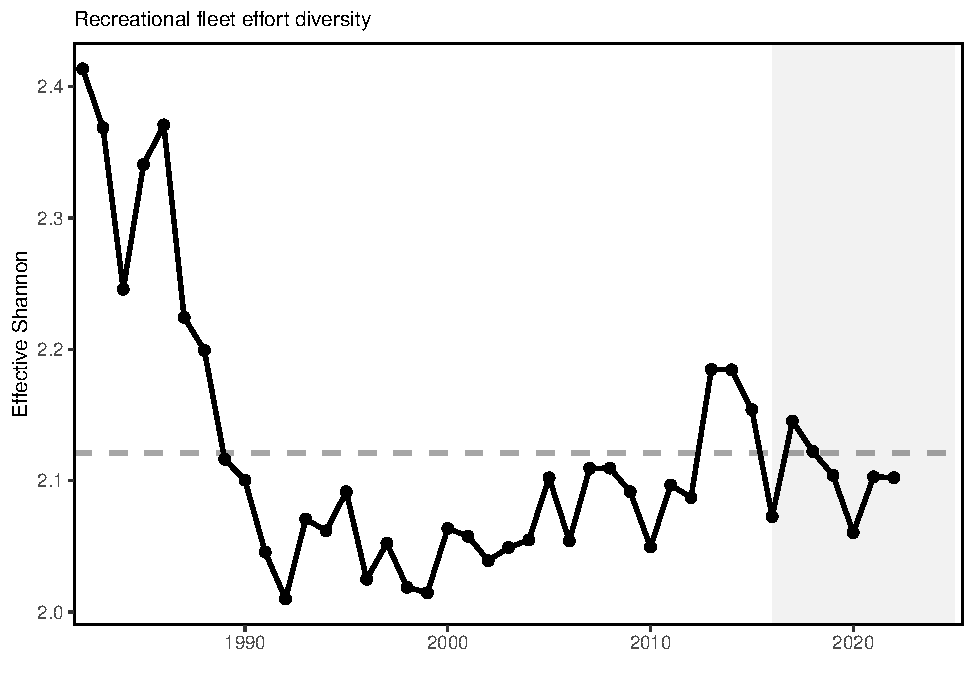
\includegraphics{NE_RiskPolicy_2025_DRAFT_files/figure-latex/rec-1} \end{center}

\end{document}
